\chapter{Improvements to basic algorithms}

\section{General pattern}

\subsection{Improving memory consumption}
As the algorithm for testing avoidance of a general pattern was described in [chapter2], it creates all possible partial mappings and checks whether at least one can be extended to a full mapping. Note that to compute all the partial mappings of some level $l$, it only uses mappings of level $l-1$; therefore, it is enough to only store partial mappings of two levels in memory.

In [chapter2] we also introduced the idea of (un)important lines for a partial mapping of level $l$ and equivalence based on not using unimportant lines at all - as they are fully bounded by other already mapped lines. When a line becomes unimportant it stays unimportant till the end of the run; as a result, we can forget where we mapped those lines to save memory. This is not as big of a deal as the previous observation was but note there are cases of patterns in which each line becomes unimportant just two levels after it gets added.

\subsection{Not mapping empty lines}
An empty line is a row or a column that does not contain any one-entries. Such a line can be mapped to any line and if the algorithm leaves space for it (which it does), we do not need to map it at all.

\subsection{Using the last changed position}
As the MCMC process works, it always changes one element of the big matrix and asks whether it still avoids the pattern. If it does not and we know that before the change it did, we are sure the changed element $[r,c]$ is a part of the pattern. It is hard to use this fact in the algorithm. It just maps one line after another and we do not know at the beginning to which line the changed position lines should be mapped.

What we can do is to enforce that neither the $r$-th line nor the $c$-th one get skipped. We will only look at the restriction for rows. The restrictions for columns are symmetrical. There are three situations we want to avoid:
\begin{itemize}
\item The first row of $P$ is mapped under the $r$-th row. This prevents any other row to be mapped to $r$-th one and we don't want that.
\item The last row of $P$ is mapped above the $r$-th row. This again prevents any other row to be mapped to $r$-th one.
\item Two adjacent rows $l,l+1$ of $P$ are mapped to $L<L'$ respectively and $L<r<L'$ which leaves no other row to be mapped to $r$.
\end{itemize}

\subsection{Line order}
An important thing, if we want the algorithm to run fast, is to choose a good line order. A line which is unimportant in level $l$ in a line order may easily be important till the nearly last level in a different order.

We choose line order to hopefully enforce two things:
\begin{itemize}
\item Make as many unimportant lines as possible. This really allows the equivalence based improvements to kick in. The more lines are unimportant the more mappings become equivalent and the faster it is to iterate through all of them.
\item Recognize hopeless partial mappings as soon as possible. A partial mapping gets extended if the line does not break the rule that there is a one-entry where it needs to be. If we map all the rows first, the rule will get broken only after we start to map columns and we probably want to find out sooner.\\
\end{itemize}
In the program a user can either choose their own custom order or one of four algorithms with different main purposes:
\begin{itemize}
\item AUTO - this one tries the other three line orders and chooses the one which shows the best performance over some iterations on a matrix. While this may sound like a good thing to use, it is only so if an initial matrix is chosen and it takes a lot of time since a lot of iterations need to be made in order to make a good sample. I would recommend not to use AUTO order at all and instead to try all the line orders by hand with a number of iterations depending on the pattern and a good initial matrix; for instance, generated with a smaller number of iterations on the same pattern and with any line order.
\item DESC - the lines are ordered in descending order depending on the number of one-entries. This follows the idea to start with the lines that are the hardest to map. Note that this algorithm does poorly if there are a lot of lines with the same number of one-entries (for example an identity matrix).
\item MAX - it orders the lines so that the maximum number of important lines throughout the levels is as small as possible. This focuses straightforwardly to having many unimportant lines, which the program does not remember.
\item SUM - it orders the lines so that the sum of the numbers of the important lines is the smallest possible throughout all levels. The purpose is the same as in the MAX order and quite often it is the case both approaches produce the same order.
\item TWO - it orders the lines so that the maximum number of important lines in two consecutive levels throughout all the levels is as small as possible. This again focuses to having many unimportant lines, which the program does not remember. The constant two is chosen due to the fact general pattern always stores two levels of partial mapping at a time.
\end{itemize}

\subsection{Mapping approaches}
The one thing the approaches we will introduce have in common is that they try to recognize those partial mappings that have no chance to be extended to a full mapping as early as possible.

While the algorithm introduced in [chapter2] finds out the partial mapping is invalid only at the time it maps two lines having a one-entry at their intersection to two lines having a zero-entry at the intersection, different approaches try to reveal the fact we would end up in the situation earlier by checking more conditions.

Imaging this as the pattern, where $0,\cdots,8$ are indices of the lines:

\centerline{\mbox{$\begin{array}{c|cccc}
&5&6&7&8 \\
\hline
0&1&1&1&1 \\
1&0&1&1&0 \\
2&1&1&0&0 \\
3&0&1&0&1 \\
4&1&1&1&0
\end{array}$}}

We are in a situation when only lines 0, 3 and 7 are mapped and line 6 is currently being mapped. Here are some mapping approaches:
\subsubsection{Enough one-entries}
In the situation above, we not only want to check there are one-entries at the intersections of line 6 with lines 0 and 3, but we also check if there are enough one-entries in lines between where lines 0 and 3 are mapped so that there is a hope we can map lines 1 and 2 there and if there is a one-entry below the line where line 3 is mapped so we can map line 4 there later.

\centerline{\mbox{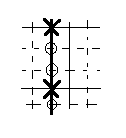
\includegraphics[width=60mm]{../img/enough_one-entries.png}}}
\subsubsection{Recursive mapping}
While we were only testing whether there are enough one-entries in between already mapped lines in the previous approach, this time, we also check whether those one-entries can be used for the lines that are intended to be mapped there. For example, when we check there is a one-entry to be used for line 1 later, we also check the line 1 can be mapped to that row, which in this situation means to also check there is a one-entry at the intersection with the line to which the line 7 is mapped.

\centerline{\mbox{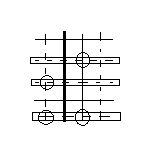
\includegraphics[width=60mm]{../img/recursive.png}}}
\subsubsection{Orthogonal bounds}
When adding line 6, we check whether there are enough one-entries on the already mapped lines orthogonal to line 6, in between line 6 and the closest mapped lines next to line 6. The same idea as in ``Enough one-entries'', but checking different lines.

\centerline{\mbox{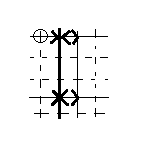
\includegraphics[width=60mm]{../img/orthogonal.png}}}
\subsubsection{Usage}
These restrictions on the added lines are not a fixed part of the program. A user can decide which approaches they want to use in the configuration file. This is due to the fact that there is no right path to choose.

In the testing that was done for a fixed pattern, we found out it is useful to use all the mentioned restrictions when generating a matrix of size $100\times100$, as it turned out to be much faster than without the restrictions. On the other hand, in the same test for a generated matrix of size $500\times500$, it was much better not to use any of those restrictions.

\subsection{Using the whole structure in the next iteration}
It may seem like a good idea to remember all the partial mappings, to propagate them to the next iteration of the MCMC process and alter them depending upon the change.

This really can be done. If the change is from zero-entry to one-entry, for each partial mapping we already have we want to try to extend it by the line that just changed and if we manage to do that we then try to extend it to a full mapping in all possible ways if it is a new mapping or do nothing if it is equivalent with a partial mapping of higher level. This can be easily done by means already used in the standard algorithm and may lead to a better performing one.

However, if the element gets changed from one-entry to zero-entry we need to go through the partial mappings and delete those that used the currently changed one-entry. This gets a bit messy as we can no longer forget unimportant lines and moreover for each partial mapping we need to remember how many partial mappings of the previous level can be extended to that one, to delete that mapping from the list if there are no longer any mappings extensible to that one.

This can all be done, but the whole thing comes with three huge inconveniences:
\begin{itemize}
\item Memory consumption - there can be a LOT of partial mappings and we need to remember them all. Of course we can still use the equivalence but we need to remember mappings of all levels.
\item The change from one-entry to zero-entry is no longer for free. If this change is done, we already know the pattern is not contained in $M$, but we still need to do a lot of work to change the structure in order to use it in the next iteration.
\item Reverting - if the change is unsuccessful (the pattern is contained) we need to revert the change which means to completely revert all changes we did to the list of partial mappings. This can be either done by making a backup copy of the whole structure and override the structure if needed, which again is very costly as the structure is huge, or we can remember what partial mappings are new and we go through all partial mappings and remove those new ones. This again means to iterate through the big structure one more time.
\end{itemize}
After realizing these issues it no longer looks useful to me to implement this version of the algorithm.

\section{Walking pattern}
While the brute force implementation of an avoid algorithm for a general pattern was improved heavily, the algorithm for a walking pattern is very fast in its nature and cannot be much better. Or can it be?

\subsection{Using the last changed position}
As the MCMC process works it always changes one element of the big matrix and asks whether it still avoids the pattern. If it does not and we know that before the change it did, we are sure the changed element is a part of the pattern. Knowing that and using the same inductive proof as we did in the proof of correctness of the avoid algorithm (see [chapter2]) it is sufficient to only recompute the part of the inner structure under the changed element and check if the last entry of the pattern can be found there.

Not only that. We also know, using the fact the structure was completely correct before the change, that if the values of both $c_v$ and $c_h$ of an element did not change, the element won't cause the element underneath it to change and we no longer have to recompute the other parts of the structure.

To use both these facts we replace the cycle through the diagonals by a simple queue, starting at the position of the last changed element and putting more positions in if the values of $c_v$ or $c_h$ are different than they were before. The function ends either when the pattern was discovered or when the queue becomes empty.

\subsection{Lazy avoid}
Lazy avoid is a variant of avoid function used when the MCMC parallelism is chosen. While all the other types of patterns have a trivial implementation of revert function, when using the walking pattern the inner structure needs to be modified even when reverting. The MCMC parallelism turned out to work much better if the revert calls are handled by the main thread (more in [chapter4]) and it requires the function to run as fast as possible so the other threads are not blocked by the call for too long. That is a reason why functions lazy revert and lazy avoid were created.

The avoid function expects the inner structure of the walking pattern (see [chapter3]) to be in a valid state and that requires some effort. To make lazy revert the fastest possible, we postpone the work until the next call of lazy avoid, meaning that lazy avoid then needs to do more things at once. It is no longer sufficient to only compute the submatrix under the position changed last as we did above, but it needs to also compute changes in the positions changed in those lazy revert calls that are postponed.

We discuss several approaches, starting with the easiest one and ending with the one that is fast and used in the final implementation.

\subsubsection{Recompute the whole structure every time}
The easiest way how to implement lazy avoid would be to always recompute the whole inner structure. In that case we do not worry which positions are correct and which are not, because every time we find the pattern, we recomputed all the entries that form it, so we know it really is there. On the other hand, if we manage to recompute the whole structure without finding the last entry of the pattern, it just is not there.

The issue is efficiency. If the whole structure was correct and there was a change of the last entry of the matrix it is sufficient to only recompute that one entry. Instead we recompute a possibly very big structure. This results in a very bad performance negating the advantage of parallel computation.
\subsubsection{Recompute only a part of the structure diagonal by diagonal}
A simple improvement would be to remember the changes done in previous calls of lazy revert and together with the change done in lazy avoid call only recompute the part of the structure that has possibly altered.

This gets a bit tricky when lazy avoid call actually discovers the pattern because we cannot be sure the rest of the structure is in a correct order. It is still possible to remember some horizontal, vertical and diagonal bounds and use them to restrict the recomputed part of the matrix. The improvement is not that significant though and we can do better.
\subsubsection{Queue of positions to recompute}
A different approach is closer to the one used in a standard avoid function. Instead of going through diagonal one after another, we have a queue of entries-to-recompute. It is no longer sufficient to have a standard queue since in different calls of lazy revert/avoid we can possibly change an entry of different priority (the higher the more important) so we need to have some kind of a priority queue. That is exactly what I tried.

Using std::priority\_queue the function had no more problems with recomputing the entries that were not influenced by the changes and used all the benefits mentioned in the previous section. But the container does not come for free and in the end I found out the price I payed for the operations on the priority queue made the whole implementation comparably slow as in the previous attempt.
\subsubsection{Two leveled queue of positions to recompute}
The final solution comes with the same idea, but a different storage type. As the priority depends upon a diagonal (two entries on the same diagonal can be recomputed in any order) we only remember a priority queue of diagonals and an array of diagonals saying whether a diagonal is already a member of the priority queue. As far as the entries are concerned for every diagonal we have a std::vector of entries-to-recompute as well as an array saying whether an entry is already a member of the vector. So finally it is the case that the storage used is not only good theoretically but as the numbers say, also practically. [reference to a table of measurements or something]

\section{Parallel computing}


\subsection{MCMC parallelism}
The first approach makes the MCMC generator parallel and it can be used with all types of patterns. While the serial MCMC generator changes one element in the generated matrix and checks whether it still avoids forbidden patterns, the parallel one counts on the fact at some point it is unlikely a change does not create a mapping of the pattern. So as it expects almost every change of one element to form a pattern, it tries to deal with those changes as fast as possible.

When the parallel version of MCMC generator is chosen and it is assigned $n$ threads, it creates $n-1$ copies of the generated matrix and assigns one thread, called worker, to each of them. The last thread, which we call the main thread, makes one change of a bit in each matrix and makes the corresponding worker check the avoidance.

The job of a worker is, when woken up, only to check if its copy of the matrix still avoids the pattern when one bit is changed. On the other hand all synchronization is left to the main thread. We still want the generator to satisfy the conditions we have for the Markov chain (more in [chapter1]) in order to generate a random matrix. To achieve that we have an ID for each task it assigns and it always waits for the task with the lowest ID to end and depending on its result it continues:
\begin{itemize}
\item success: If the task with the lowest ID is successful, we can propagate the changed bit into the generated matrix. Also, since all other threads expected this one to fail, they compute a change that will never be propagated to the generated matrix and therefore is useless. What we do with that is we stop all the workers that compute a task with higher ID, revert the changes they made on their matrices and we synchronize the change computed by the successful thread. After all of this is done, all the matrices are the same.
\item fail: If the task with the lowest ID is not successful, there is no change to propagate to the generated matrix. This still makes a valid iteration of the MCMC process though and since all the other threads expected this one to fail, they compute correct changes.
\end{itemize}
In both cases a new task is then assigned to the worker.

\subsubsection{Speculative computing}
It may easily happen that a task not having the lowest ID ends first. In that case we could just wait until it has the lowest ID and process it later. This would be pretty costly though. Instead we process the task immediately, just as described for the task with the lowest ID, but we don't propagate the changes to the generated matrix and we do not stop the workers processing a task with lower ID. This gets a bit tricky when the task succeeds. Not only we revert all the changes computed by tasks with higher ID and synchronize the changes computed by the worker (we would do that even if waiting for the task to have the lowest ID), but it might happen a task with even lower ID succeeds as well. This leads to a need of reverting the synchronizations we made. Luckily this is the only precarious situation we may encounter and it is not that hard to deal with it.

The way we deal with these inconveniences is described in [chapter5] and should be clear from the code itself.

\subsubsection{Reverting and synchronizing in the main thread}
The speculative computing discussed above is not the only improvement
we can make. It turns out that it is costly to wake a thread so it computes a trivial function, sets a few atomic variables and falls asleep again. This happens a lot. Every time a call of avoid succeeds it makes other workers revert their changes and synchronize the successful change, which are both trivial functions.

To workaround this problem we make a theoretically bad decision which has very nice practical results. All the reverts and synchronizations are computed by the main thread instead of by an appropriate worker. There is no problem with concurrency because the worker is always asleep when a revert or sync calls are to be assigned and using the fact those calls are really trivial, it does not make the rest of threads wait for the main thread for too long while it computes changes.